%\subsection{Durchführung}
%\label{sec:Durchführung}
\section{Wheatstonebrücke}
\subsection{Durchführung}
Abbildung \ref{fig:1} zeigt den systematischen Aufbau einer Wheatstonebrücke.
\begin{figure}[H]
  \centering
  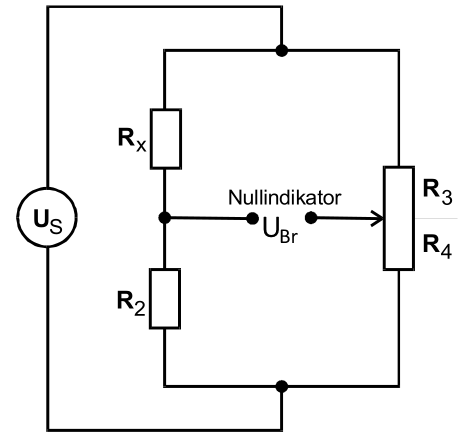
\includegraphics[height=6cm]{wheat.png}
  \caption{Wheatstonebrücke \cite{sample}}
  \label{fig:1}
\end{figure}
Sie besteht aus jeweils zwei parallel zueinander geschalteten Widerständen $R_x$ und $R_3$, und $R_2$ und $R_4$.
Es wird die Potentialdifferenz $U_{\text{br}}$ zwischen den beiden Punkten nach jeweils dem ersten Widerstand abgegriffen.
Bei dieser mit Wechselstrom betriebenen Schaltung wird das Verhältnis von $R_3$ zu $R_4$ nun solange variiert bis die Brückenspannunng $U_{\text{Br}}$ ihr Minimum erreicht hat.
Somit kann $R_x$ bestimmt werden.
Es werden zwei unbekannte Widerstände $R_x$ mit jeweils drei verschiedenen $R_2$ ermittelt.
\subsection{Auswertung}
Die gemessenen Daten sind in den Tabellen \ref{tab:1} für Wert 14 und \ref{tab:2} für Wert 11 abgebildet.
Der relative Fehler vom Verhältnis $\frac{R_3}{R_4}$ beträgt $0.5\%$, der relative Fehler von $R_2$ $0.2\%$. \cite{sample}
\begin{table}
  \centering
  \caption{Messdaten für R = Wert 14}
  \label{tab:1}
  \sisetup{table-format=3.4}
  \begin{tabular}{c c c c}
    \toprule
    {$R_2 [\si{\ohm}]$} & {$\increment R_2 [\si{\ohm}]$} & {$\frac{R_3}{R_4}$} & {$\increment \frac{R_3}{R_4}$} \\
    \midrule
    \input{build/wheat1tabelle.tex}
    \bottomrule
  \end{tabular}
\end{table}


\begin{table}
  \centering
  \caption{Messdaten R = Wert11}
  \label{tab:2}
  \sisetup{table-format=3.4}
  \begin{tabular}{c c c c}
    \toprule
    {$R_2 [\si{\ohm}]$} & {$\increment R_2 [\si{\ohm}]$} & {$\frac{R_3}{R_4}$} & {$\increment \frac{R_3}{R_4}$} \\
    \midrule
    \input{build/wheat2tabelle.tex}
    \bottomrule
  \end{tabular}
\end{table}
Über den in der Theorie genannten Zusammenhang \ref{eqn:1} ergibt sich für den unbekannten Widerstand
\begin{equation}
  R_x = R_2 \frac{R_3}{R_4}.
\end{equation}
Somit errechnen sich die jeweiligen Messwerte zu $R_{14}$ und $R_{11}$ zu
\begin{align*}
  R_{14,1}   &= \input{build/wheat/wheat.R14_1.tex} & R_{11,1} &= \input{build/wheat/wheat.R11_1.tex},\\
  R_{14,2}   &= \input{build/wheat/wheat.R14_2.tex} & R_{11,2} &= \input{build/wheat/wheat.R11_2.tex},\\
  R_{14,3}   &= \input{build/wheat/wheat.R14_3.tex} & R_{11,3} &= \input{build/wheat/wheat.R11_3.tex}.
\end{align*}
Für die Fehlerrechnung wird bei der vorliegenden Rechnung und bei allen folgenden Rechnungen das Gaußsche Fehlerfortpflanzungsgesetz
\begin{equation}
\increment{f} = \sqrt{\Bigl(\frac{\partial f}{\partial x_1}\increment{x_1}\Bigr)^2 + \Bigl(\frac{\partial f}{\partial x_2}\increment{x_2}\Bigr)^2 + \dotsc + \Bigl(\frac{\partial f}{\partial x_n}\increment{x_n}\Bigr)^2}
\end{equation}
für eine Funktion $f(x_1,x_2, \dotsc ,x_n)$, bei der die Größen $x_1, x_2, \dotsc , x_n$ voneinander unabhängig sind, verwendet.
Dementprechend berechnet sich der Fehler von $R_x$ zu
\begin{equation}
\increment{R_x} = \sqrt{\frac{R_3^2}{R_4^2} \cdot \increment{R_2}^2 + R_2^2 \cdot \Bigl(\increment{\frac{R_3}{R_4} }\Bigr)^2}.
  \label{eqn:fehler1}
\end{equation}
Die daraus errechneten Mittelwerte ergeben
\begin{align*}
  R_{14}   &= \input{build/wheat/wheat.R14m.tex},\\
  R_{11}   &= \input{build/wheat/wheat.R11m.tex}.
\end{align*}

\section{Kapazitätsmessbrücke}
\subsection{Durchführung}
Mit der Kapazitätsmessbrücke kann die Kapazität und der Widerstand eines unbekannten Kondensatorelements berechnet werden.
Die Abbildung \ref{fig:2} zeigt eine solche Schaltung.
\begin{figure}[H]
  \centering
  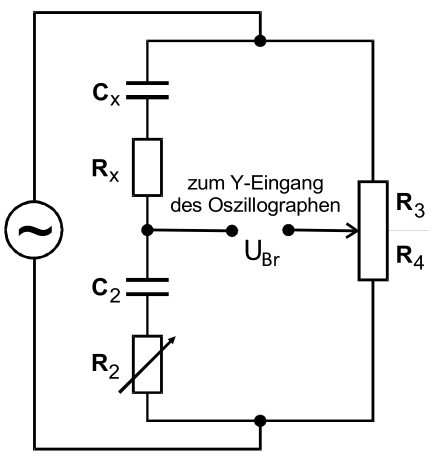
\includegraphics[height=6cm]{kapa.png}
  \caption{Kapazitätsmessbrücke \cite{sample}}
  \label{fig:2}
\end{figure}
Sie unterscheidet sich von der Wheatstonebrücke nur darin, dass hier anstelle von $R_x$ eine unbekannte R/C-Kombination oder eben ein unbekannter verlustbehafteter Kondensator eingebaut und betrachtet wird.
Zusätzlich wird mit einem festen Kondensator $C_2$ und einem variablen Widerstand $R_2$ abgeglichen.
Es werden nun $R_2$ und das Verhältnis von $R_3$ und $R_4$ solange nacheinander variiert, bis das Minimum der Brückenspannung $U_{\text{Br}}$ auf dem Oszilloskop beobachtet wird.
Auf diese Weise werden die Kapazitäten und Widerstände einer R/C-Kombination, sowie von zwei unbekannten verlustbehafteten Kondensatoren bestimmt.
Es wird jeweils dreimal mit verschiedenen Kondensatoren $C_2$ gemessen.

\subsection{Auswertung}
Die gemessenen Daten sind in Tabelle \ref{tab:3} für die RC-Kombination 8, in der Tabelle \ref{tab:4} für den Kondensator 3 und in der Tabelle \ref{tab:5} für den Kondensator 1 angegeben.
Der relative Fehler von $C_2$ beträgt $0.2\%$, der relative Fehler von $\frac{R_4}{R_3}$ beträgt $0.5\%$ und der relative Fehler von $R_2$ beträgt $3\%$. \cite{sample}
\begin{table}[H]
  \centering
  \caption{Messdaten R/C = Wert 8}
  \label{tab:3}
  \sisetup{table-format=3.4}
  \begin{tabular}{c c c c c c}
    \toprule
    {$C_2 [\si{\nano\farad}]$} & {$\increment C_2 [\si{\nano\farad}]$} & {$R_2 [\si{\ohm}]$} & {$\increment R_2 [\si{\ohm}]$} & {$\frac{R_4}{R_3}$} & {$\increment \frac{R_4}{R_3}$} \\
    \midrule
    \input{build/kapa1tabelle.tex}
    \bottomrule
  \end{tabular}
\end{table}
\begin{table}[H]
  \centering
  \caption{Messdaten C = Wert 3}
  \label{tab:4}
  \sisetup{table-format=3.4}
  \begin{tabular}{c c c c c c}
    \toprule
    {$C_2 [\si{\nano\farad}]$} & {$\increment C_2 [\si{\nano\farad}]$} & {$R_2 [\si{\ohm}]$} & {$\increment R_2 [\si{\ohm}]$} & {$\frac{R_4}{R_3}$} & {$\increment \frac{R_4}{R_3}$} \\
    \midrule
    \num{399} & \num{0.8} & \num{0} & \num{0} & \num{1.045} & \num{0.005} \\
    \num{750} & \num{2} & \num{0} & \num{0} & \num{0.558} & \num{0.003} \\
    \num{597} & \num{1} & \num{0} & \num{0} & \num{0.698} & \num{0.003} \\
    \bottomrule
  \end{tabular}
\end{table}
\begin{table}[H]
  \centering
  \caption{Messdaten C = Wert 1}
  \label{tab:5}
  \sisetup{table-format=3.4}
  \begin{tabular}{c c c c c c}
    \toprule
    {$C_2 [\si{\nano\farad}]$} & {$\increment C_2 [\si{\nano\farad}]$} & {$R_2 [\si{\ohm}]$} & {$\increment R_2 [\si{\ohm}]$} & {$\frac{R_4}{R_3}$} & {$\increment \frac{R_4}{R_3}$} \\
    \midrule
    \input{build/kapa3tabelle.tex}
    \bottomrule
  \end{tabular}
\end{table}
Aus der Gleichung \ref{eqn:bed1} ergibt sich sofort der Zusammenhang
\begin{equation}
  R_x = R_2 \frac{R_3}{R_4}
\end{equation}
sowie aus Gleichung \ref{eqn:bed2} der Zusammenhang
\begin{equation}
  C_x = C_2 \frac{R_4}{R_3}
\end{equation}
für die abgeglichene Wechselstrombrücke.
Es folgen somit für die Kapazitäten und Widerstände der Kondensatoren aus den einzelnen Messungen
\begin{align*}
  C_{8,1}   &= \input{build/kapa/kapa.C8_1.tex} & R_{8,1} &= \input{build/kapa/kapa.R8_1.tex}\\
  C_{8,2}   &= \input{build/kapa/kapa.C8_2.tex} & R_{8,2} &= \input{build/kapa/kapa.R8_2.tex}\\
  C_{8,3}   &= \input{build/kapa/kapa.C8_3.tex} & R_{8,3} &= \input{build/kapa/kapa.R8_3.tex}
\end{align*}
\begin{align*}
  C_{3,1}   &= \input{build/kapa/kapa.C3_1.tex} & R_{3,1} &= \input{build/kapa/kapa.R3_1.tex}\\
  C_{3,2}   &= \input{build/kapa/kapa.C3_2.tex} & R_{3,2} &= \input{build/kapa/kapa.R3_2.tex}\\
  C_{3,3}   &= \input{build/kapa/kapa.C3_3.tex} & R_{3,3} &= \input{build/kapa/kapa.R3_3.tex}
\end{align*}
\begin{align*}
  C_{1,1}   &= \input{build/kapa/kapa.C1_1.tex} & R_{1,1} &= \input{build/kapa/kapa.R1_1.tex}\\
  C_{1,2}   &= \input{build/kapa/kapa.C1_2.tex} & R_{1,2} &= \input{build/kapa/kapa.R1_2.tex}\\
  C_{1,3}   &= \input{build/kapa/kapa.C1_3.tex} & R_{1,3} &= \input{build/kapa/kapa.R1_3.tex}
\end{align*}
Die Fehler bestimmen sich analog zu der in \ref{eqn:fehler1} angegebenen Fehlerformel.
Als Mittelwerte ergeben sich somit
\begin{align*}
  C_{8}   &= \input{build/kapa/kapa.C8m.tex} & R_{8} &= \input{build/kapa/kapa.R8m.tex}\\
  C_{3}   &= \input{build/kapa/kapa.C3m.tex} & R_{3} &= \input{build/kapa/kapa.R3m.tex}\\
  C_{1}   &= \input{build/kapa/kapa.C1m.tex} & R_{1} &= \input{build/kapa/kapa.R1m.tex}
\end{align*}
für die Kapazitäten und Widerstände der jeweiligen Bauteile.

\section{Induktivitätsmessbrücke}
\subsection{Durchführung}
Die Induktivitätsmessbrücke, dargestellt in Abbildung \ref{fig:3}, funktioniert analog zur Kapazitätsmessbrücke \ref{fig:2}.
\begin{figure}[H]
  \centering
  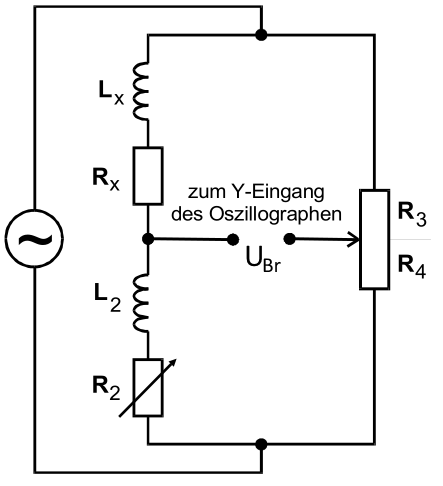
\includegraphics[height=6cm]{indu.png}
  \caption{Induktivitätsmessbrücke \cite{sample}}
  \label{fig:3}
\end{figure}
Anstelle der Kondensatoren werden hier jedoch die Spule $L_2$ und eine LR-Kombination eingebaut.
Es gilt dasselbe Messverfahren wie bei der Kapazitätsmessbrücke, um diesmal die Werte von nur einer unbekannten LR-Kombination zu ermitteln.
$L_2$ wird dabei zweimal variiert.
\subsection{Auswertung}
Die Messdaten für die Bestimmung der unbekannten LR-Kombination 19 werden in Tabelle \ref{tab:6} angegeben.
Der relative Fehler von $L_2$ beträgt $0.2\%$, der relative Fehler von $\frac{R_3}{R_4}$ beträgt $0.5\%$ und der relative Fehler von $R_2$ beträgt $3\%$. \cite{sample}
\begin{table}
  \centering
  \caption{Messdaten LR = Wert 19}
  \label{tab:6}
  \sisetup{table-format=3.4}
  \begin{tabular}{c c c c c c}
    \toprule
    {$L_2 [\si{\milli\henry}]$} & {$\increment L_2 [\si{\milli\henry}]$} & {$R_2 [\si{\ohm}]$} & {$\increment R_2 [\si{\ohm}]$} & {$\frac{R_3}{R_4}$} & {$\increment \frac{R_3}{R_4}$} \\
    \midrule
    \input{build/indu1tabelle.tex}
    \bottomrule
  \end{tabular}
\end{table}

Aus der Gleichung \ref{eqn:bed1} ergibt sich sofort der Zusammenhang
\begin{equation}
  R_x = R_2 \frac{R_3}{R_4}
\end{equation}
sowie aus Gleichung \ref{eqn:bed2} der Zusammenhang
\begin{equation}
  L_x = L_2 \frac{R_3}{R_4}
\end{equation}
für verschwindene Brückenspannung $U_Br$.
Für die Induktivität sowie den Widerstand der Spule ergeben sich für die beiden Messungen jeweils
\begin{align*}
  L_{19,1}   &= \input{build/indu/indu.L19_1.tex} & R_{19,1} &= \input{build/indu/indu.R19_1.tex}\\
  L_{19,2}   &= \input{build/indu/indu.L19_2.tex} & R_{19,2} &= \input{build/indu/indu.R19_2.tex}
\end{align*}
wobei die Fehler analog zur Fehlerformel \ref{eqn:fehler1} bestimmt werden.
Als Mittelwerte ergeben sich
\begin{align*}
  L_{19}   &= \input{build/indu/indu.L19m.tex} & R_{19} &= \input{build/indu/indu.R19m.tex}.
\end{align*}

\section{Maxwell-Brücke}
\subsection{Durchführung}
Da bei der Induktivitätsmessbrücke auf eine Spule zur Berechnung der unbekannten Induktivität zurückgegriffen wird, diese aber zumeist bei niedrigen Frequenzen hohe Verluste besitzt, ist es besser anstelle einer Spule einen möglichst verlustarmen Kondensator zu verwenden.
Dies wird bei der Maxwell-Brücke, Abbildung \ref{fig:4}, realisiert.
\begin{figure}[H]
  \centering
  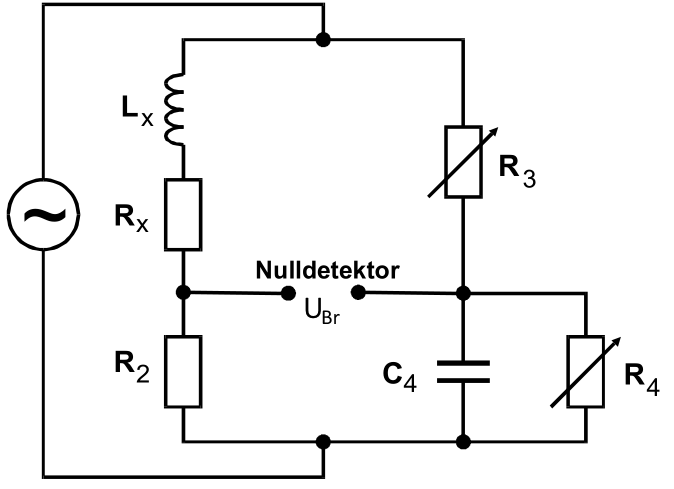
\includegraphics[height=6cm]{max.png}
  \caption{Maxwell-Brücke \cite{sample}}
  \label{fig:4}
\end{figure}
Die Abgleichelemente sind hier die variablen Widerstände $R_3$ und $R_4$, wobei der Kondensator $C_4$ parallel zu $R_4$ geschaltet wird.
Dabei soll dieselbe L/R-Kombination 19 untersucht werden, indem $R_3$ und $R_4$ nacheinander variiert werden, sodass die Brückenspannung $U_{\text{Br}}$ minimal wird.
Es wird dreimal mit verschiedenen Widerständen $R_2$ gemessen.
\subsection{Auswertung}
Die Messwerte für die drei Messungen mit jeweils verschiedenen $R_2$ werden in Tabelle \ref{tab:7} angegeben.
Der relativen Fehler von $R_3$ sowie $R_4$ betragen $3\%$, die Fehler von $R_2$ sowie $C_4$ betragen $0.2\%$. \cite{sample}
\begin{table}
  \centering
  \caption{Messdaten LR = Wert 19}
  \label{tab:7}
  \sisetup{table-format=3.4}
  \begin{tabular}{c c c c c c c c c c}
    \toprule
    {$C_4 [\si{\nano\farad}]$} & {$\increment C_4 [\si{\nano\farad}]$} & {$R_4 [\si{\ohm}]$} & {$\increment R_4 [\si{\ohm}]$} & {$R_3 [\si{\ohm}]$} & {$\increment R_3 [\si{\ohm}]$} & {$R_2 [\si{\ohm}]$} & {$\increment R_2 [\si{\ohm}]$} & {$\frac{R_3}{R_4}$} & {$\increment \frac{R_3}{R_4}$} \\
    \midrule
    \input{build/max1tabelle.tex}
    \bottomrule
  \end{tabular}
\end{table}
Aus der Gleichung \ref{eqn:bed1} folgt der Zusammenhang
\begin{equation}
  R_x = R_2 \frac{R_3}{R_4}
\end{equation}
und aus der Gleichung \ref{eqn:bed2} der Zusammenhang
\begin{equation}
  L_x = C_4R_3R_2.
\end{equation}
Aus der Gaußschen Fehlerfortpflanzung folgt für den Fehler von $R_x$
\begin{equation}
\increment{R_x} = \sqrt{\Bigl( \frac{R_3}{R_4} \cdot \increment{R_2} \Bigr)^2 + \Bigl( \frac{R_2}{R_4} \cdot \increment{R_3}\Bigr)^2 + \Bigl( \frac{R_2 R_3}{R_4^2} \increment{R_4} \Bigr)^2}
  \label{eqn:fehler1}
\end{equation}
sowie für den Fehler von $L_x$
\begin{equation}
\increment{L_x} = \sqrt{\Bigl( R_3 R_2 \increment{C_4} \Bigr)^2 + \Bigl( C_4 R_2 \increment{R_3} \Bigr)^2 + \Bigl( C_4 R_3 \increment{R_2} \Bigr)^2}.
  \label{eqn:fehler1}
\end{equation}
Hieraus ergeben sich aus den drei Messungen für die Induktivität sowie den Widerstand vom Wert 19
\begin{align*}
  L_{19,1}   &= \input{build/max/max.L19_1.tex} & R_{19,1} &= \input{build/max/max.R19_1.tex}\\
  L_{19,2}   &= \input{build/max/max.L19_2.tex} & R_{19,2} &= \input{build/max/max.R19_2.tex}\\
  L_{19,3}   &= \input{build/max/max.L19_3.tex} & R_{19,3} &= \input{build/max/max.R19_3.tex}.
\end{align*}
Als Mittelwert für den Wert 19 folgt somit
\begin{align*}
  L_{19}   &= \input{build/max/max.L19m.tex} & R_{19} &= \input{build/max/max.R19m.tex}.
\end{align*}

\section{Wien-Robinson-Brücke}
\subsection{Durchführung}
Bei den obigen Schaltungen ist ein Abgleich bei beliebigen Frequenzen möglich.
Bei der Wien-Robinson-Brücke \ref{fig:5} hingegen ist ein Abgleich nur bei einer bestimmten Frequenz möglich, die untersucht werden soll.
\begin{figure}[H]
  \centering
  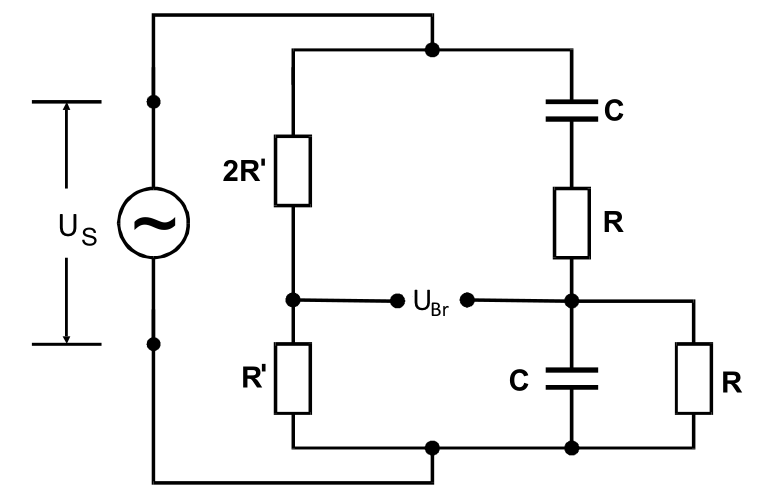
\includegraphics[height=6cm]{wien.png}
  \caption{Wien-Robinson-Brücke \cite{sample}}
  \label{fig:5}
\end{figure}
Dabei wird die Frequenz $v$ der Speisespannung $U_{\text{S}}$ in um die Minimalbrückenspannung kleiner werdenden Abständen variiert und die jeweilige entstehende Brückenspannung $U_{\text{Br}}$ notiert.
Die Frequenz befindet sich in einem Bereich von $\SI{20}{\hertz}$ bis $\SI{30}{\kilo\hertz}$.
\subsection{Auswertung}

\begin{table}
  \centering
  \caption{Messdaten Frequenzmessung.}
  \label{tab:8}
  \sisetup{parse-numbers=false}
  \begin{tabular}{
    S[table-format=1.3]
    S[table-format=1.3]
    @{${}{}$}
    %S[table-format=1.2]
    @{\hspace*{3em}\hspace*{\tabcolsep}}
    S[table-format=1.3]
    S[table-format=1.3]
    @{${}{}$}
    %S[table-format=1.2]
  }
    \toprule
    {$v \:/\: \si{\hertz}$} & {$U_{\text{Br}} \:/\: \si{\volt}$} &
    {$v \:/\: \si{\hertz}$} & {$U_{\text{Br}} \:/\: \si{\volt}$} \\
    \midrule
    \input{build/frequenztabelle.tex}
    \bottomrule
  \end{tabular}
\end{table}


\begin{equation}
  f(v) = \frac{U_{\text{Br}}}{U_{\text{S}}} = \sqrt{\frac{1}{9} \frac{\left(\Omega²-1 \right)²}{\left(1-\Omega² \right)²+9\Omega²}}
\end{equation}


\begin{figure}[H]
  \centering
  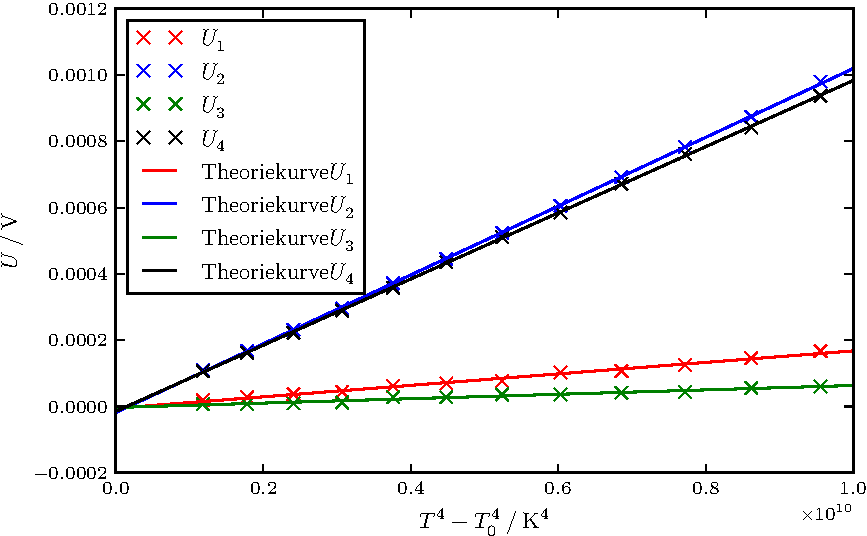
\includegraphics[height=10cm]{plot.pdf}
  \caption{Frequenzmessergebnisse}
  \label{fig:6}
\end{figure}
